\chapter{Succinct de Bruijn Graphs Blog Post}

This post will give a brief explanation of a Succinct implementation for storing \emph{de Bruijn graphs},\footnote{\url{http://en.wikipedia.org/wiki/De_Bruijn_graph}} which is recent (and continuing) work I have been doing with Sadakane.

Using our new structure, we have squeezed a graph for a human genome (which took around 300 GB of memory if using previous representations) down into 2.5 GB. In addition, the construction method allows much of the work to be done on disk. Your computer might not have 300 GB of RAM, but you might have 2.5 GB of RAM and a hard disk.

I have given a talk about this a few times, so I've been itching to write it up as a blog post (if only to shamelessly plug my blog at conferences). However, since it is a lowly blog post, I won't give attention to the gory details, nor provide any experimental results. But this post is merely to \emph{communicate the approach}. Feel free to check out our conference paper~\cite{bowe}, and stay tuned for the journal paper.

In this blog post, I will first give an introduction to de Bruijn graphs (Section~\ref{bl-sec:dbg}) and how they are used in DNA assembly (Section~\ref{bl-sec:dna}). Then I will briefly explain some previous implementations (Section~\ref{bl-sec:pre}) before reaching the main topic of this post: our new succinct representation (Section~\ref{bl-sec:our}). The explanation first explains some preliminaries, such as how we were inspired by the Burrows Wheeler Transform (Section~\ref{bl-sec:bur}), and what rank and select are (Section~\ref{bl-sec:ras}), which are required to understand the construction method (Section~\ref{bl-sec:con}), and traversal interface (Section~\ref{bl-sec:int}) respectively.

For those following along at home, I have implemented a demo version in Python.\footnote{\url{https://github.com/alexbowe/debby/blob/0.1.1/debby.py}} It doesn't use efficient implementations of rank and select, nor provide any compression -- it is merely meant to demonstrate the key ideas with (hopefully) readable high level code. An optimised version will be made available at some point.

Okay, here we go\ldots

\section{De Bruijn Graphs}\label{bl-sec:dbg}

De Bruijn graphs are a beautifully simple, yet useful combinatoric object which I challenge you not to lose sleep over.

Since their discovery around 1946, they have been used in a variety of applications, such as encryption, psychology, chess and even card tricks. Quite recently they have become a popular data structure for DNA assembly of short read data.

They are defined as a directed graph, where each node $u$ represents a fixed-length string (say, of length $k$, and an edge exists from $u$ to $v$ iff they overlap by $k-1$ symbols. That is, $u[2..k]=v[1..k-1]$.

Let's make this concrete with a diagram:

\medskip\centerline{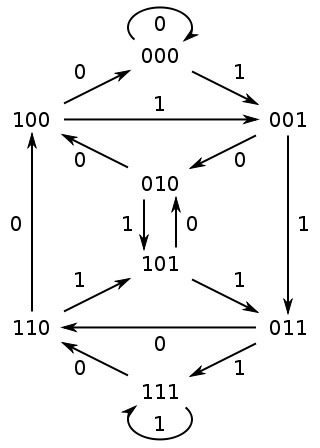
\includegraphics[width=0.4\textwidth]{23debruijn}}\medskip

Doesn't this just \emph{feel good} to look at? Now tilt your head and look at it this way: it is essentially a \emph{Finite State Machine}\footnote{\url{https://en.wikipedia.org/wiki/Finite-state_machine}} with additional bounded memory of the last $k$ visited states, if you added a few more states to allow for incomplete input at the start. For example, if X represents blank input, from a starting state XXX we might have the transition chain: $\rm XXX \to XX1 \to X10 \to 101$ (which is already a node in the graph). Put this way, it is easy to see that the $k$ previous edges define the current node. This perspective will make things easier to understand later, I promise.

Still with me? Good. Then let's also consider that if one node is defined by a $k$-length string, then a \emph{pair of nodes} (i.e.\ an edge) can be identified by a $k+1$ length string, since they overlap and differ by 1 symbol. This will also be important later.

And of course, this can be extended to larger alphabet sizes than binary (say, 4\ldots).

\section{DNA Assembly}\label{bl-sec:dna}

First suggested in 2001 by Pevzner et al.~\cite{PevTan01}, we can use de Bruijn graphs to represent a network of overlapping \emph{short read data}.

The long and short of it (heh heh) is that a DNA molecule is currently too difficult to sequence (that is, read it into a computer) in its entirety. Special methods must be used so we can sequence parts of the molecule, and hand off the putting-back-together process (assembly) to an algorithm.

One current popular sequencing method is \emph{shotgun sequencing}, which clones the genome a bunch of times, then randomly breaks each clone into short segments. If we can sequence the short segments, then the fact that we randomly cut up the clones should lead us to have overlapping reads. Of course it is a bit more complicated than this in reality, but this is the essence of it.

\medskip\centerline{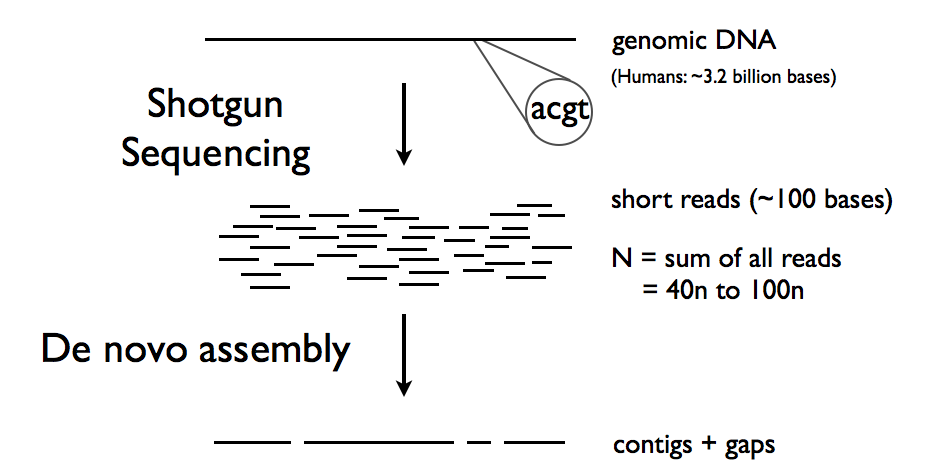
\includegraphics[width=0.7\textwidth]{shotgun}}\medskip

We then move a sliding window over each read, outputing overlapping $k$-mers (the $k$-length strings), which we use to create our de Bruijn graph.

About now mathematicians among you might raise your hand to tell me ``that may not technically yield a de Bruijn graph''. That's correct -- in Bioinformatics the term ``de Bruijn graph'' is overloaded to mean a subgraph. Even though genomes are long strings, most genomes won't have \emph{every single $k$-mer} present, and there is usually repeated regions. This means our data will be sparse.

Consider the following contrived example. Take the sequence TACGACGTCGACT. If we set $k=3$, our $k$-mers will be TAC, ACG, CGA, and so on. We would end up with this de Bruijn graph:

\medskip\centerline{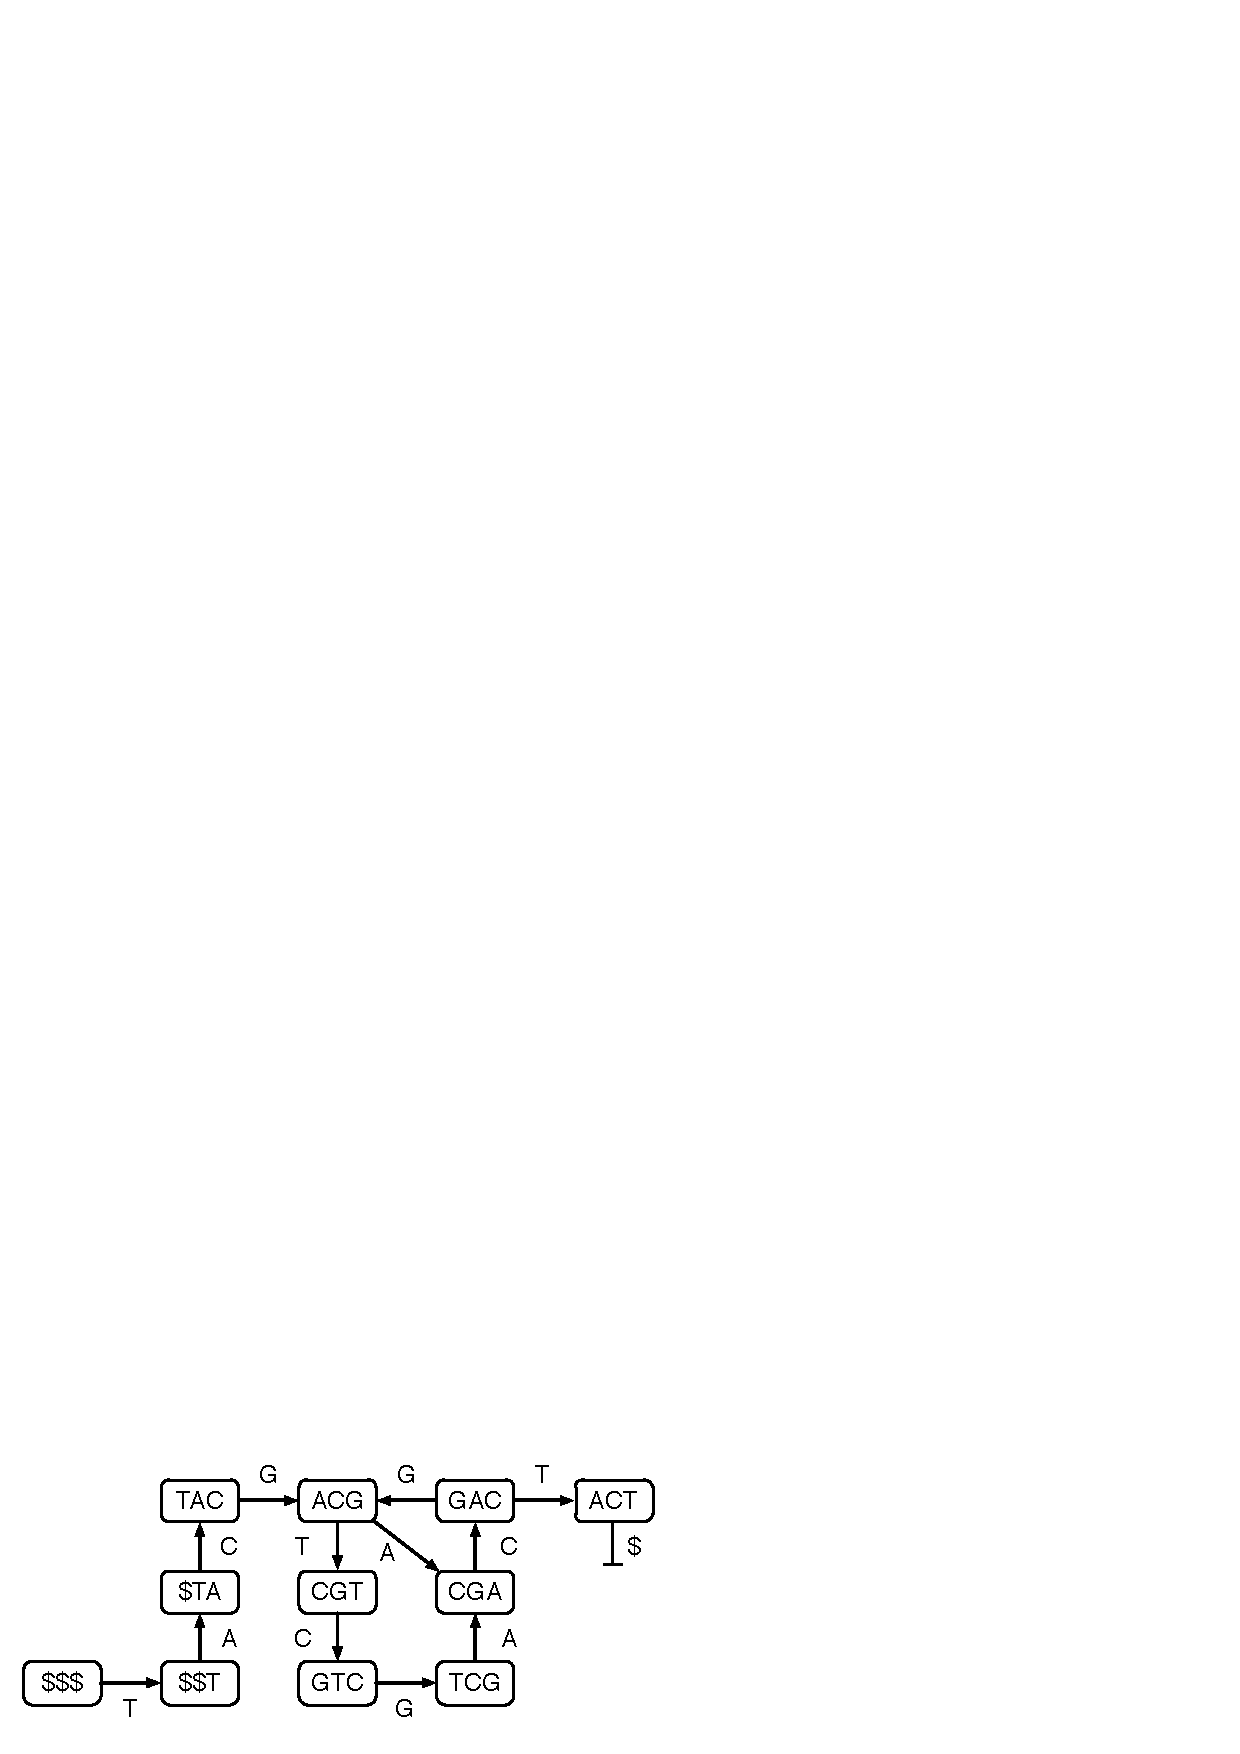
\includegraphics[width=0.6\textwidth]{graph}}\medskip

After we construct the graph from the reads, assembly becomes finding the ``best'' contiguous regions. The jury is still out on what the best method is (or what ``best'' even means); the point of this post isn't about assembly, but our implementation of the data structure and how it provides all required navigation options to implement any traversal method. I recommend reading this primer from Nature\footnote{\url{http://www.cs.ucdavis.edu/~gusfield/cs225w12/deBruijn.pdf}} if you want to get deeper into this.

Even though this is only a de Bruijn \emph{subgraph}, these things still grow pretty big. It is worthwhile considering how to handle this scalability issue, if only to reduce hardware requirements of sequencing (thus proliferating personal genomics), and potentially improve traversal speed (due to better memory locality). Increased efficiency might also enable richer multiple-genomic analysis.

\section{Previous Representations}\label{bl-sec:pre}

One of the first approaches to this was to scale ``horizontally''. Simpson et al.~\cite{Simpson:2009} introduced ABySS in 2009. The graph for reads from a human genome (HapMap: NA18507),\footnote{\url{ftp://ftp.ddbj.nig.ac.jp/ddbj_database/dra/fastq/SRA010/SRA010896/SRX016231/}} which used a distributed hash table, reached 336 GB.

In 2011, Conway and Bromage~\cite{ConBro11} instead approached this problem from a ``vertical'' scaling perspective (that is, scaling to make better use of a single system's resources), by using a sparse bitvector (by Okanohara and Sadakane~\cite{OkaSad07}) to represent the $(k+1)$-mers (the edges), and used \emph{rank and select} (to be described shortly in Section~\ref{bl-sec:ras}) to traverse it. As a result, their representation took 32 GB for the same data set.

Minia, by Cikhi and Rizk (2012)~\cite{wabi}, proposed yet another approach by using a \emph{bloom filter}\footnote{\url{http://en.wikipedia.org/wiki/Bloom_filter}} (with additional structure to avoid false positive edges that would affect the assembly). They traverse by generating possible edges and testing for it in the bloom filter. Using this approach, the graph was reduced to 5.7 GB.

\section{Our Succinct Representation}\label{bl-sec:our}

As stated, we were able to represent the same graph in 2.5 GB (after some further compression techniques, which I will save for a future post).

The key insight is that the edges define overlapping node labels. This is similar to that of Conway and Bromage, although they have some redundancy, since some \emph{nodes} are represented more times than necessary.

We further exploit the \emph{mutual information}\footnote{\url{https://en.wikipedia.org/wiki/Mutual_information}} of edges by taking inspiration from the Burrows Wheeler Transform~\cite{BurWhe94}.

\subsection{Inspiration from the Burrows Wheeler Transform}\label{bl-sec:bur}

The Burrows Wheeler Transform~\cite{BurWhe94} is a reversible string permutation that can be searched directly and has the admirable quality of having long strings of repeated characters (great for compression). The easiest way to calculate the BWT of a string is to sort each symbol by their prefixes in colex order (that is, alphabetic order of the reverse of the string, not reverse alphabetic!) More information can be found on Wikipedia\footnote{\url{http://en.wikipedia.org/wiki/Burrows-Wheeler_transform}} and this Dr. Dobbs\footnote{\url{http://marknelson.us/1996/09/01/bwt/}} article.

The XBW is a generalisation of the BWT that applies to rooted, labeled trees~\cite{FLMM09}. The idea is that instead of taking all suffixes, we sort all paths from the root to each node, and support tree navigation (since it isn't a linearly shaped string) with auxiliary bit vectors indicating which edges are leaves, and which are the last edges (of their siblings) of internal nodes.

I won't go into detail, but in the next section you should be able to see glimpses of these two ideas.

\subsection{Construction}\label{bl-sec:con}

The simplest construction method\footnote{The paper also describes an online construction method (where we can update by appending), and an iterative method that builds the $k$-dimensional de Bruijn graph from an existing $(k–1)$-dimensional de Bruijn graph.} is to take every $<\rm node, edge>$ pair and sort them based on the reverse of the node label (colex order), removing duplicates\footnote{We currently use an external merge sort, but intend to optimise as this is where Minia beats us time-wise.}. We also padding to ensure every node has an incoming and an outgoing edge. This maintains the fact that a node is defined by its previous $k$ edges. An example can be seen below:

\medskip\centerline{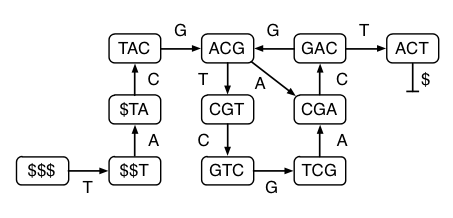
\includegraphics[width=0.7\textwidth]{graph-padded}\hfill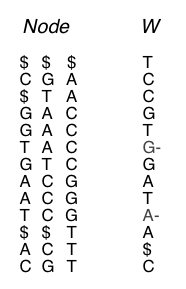
\includegraphics[width=0.26\textwidth]{arrays-1}}\medskip
 
You may have spotted that we have flagged some edges with a minus symbol. This is to disambiguate identically labelled incoming edges -- edges that exit separate nodes, but have the same symbol, and thus enter the same node. In the example below, the nodes ACG and CGA both have two incoming edges.

\medskip\centerline{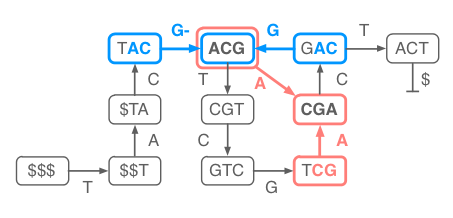
\includegraphics[width=0.7\textwidth]{edges}\hfill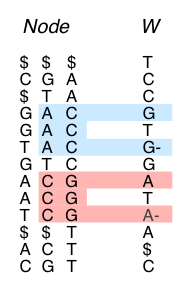
\includegraphics[width=0.26\textwidth]{array-edges-flags}}\medskip
 
Notice that each outgoing edge is stored contiguously? We include a bit vector to represent whether an edge is the \emph{last} edge exiting a node. This means that each node will have a sequence of zero-or-more 0-bits, followed by a single 1-bit.

\medskip\centerline{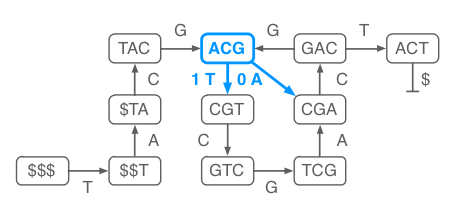
\includegraphics[width=0.7\textwidth]{last-edges}\hfill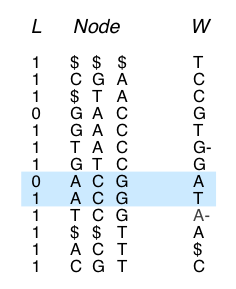
\includegraphics[width=0.3\textwidth]{last-array}}\medskip
 
Since a $1$ in the $L$ vector identifies a unique node, we can use this vector (and \emph{select}, explained shortly in Section~\ref{bl-sec:ras}) to index nodes, whereas standard array indexing points to edges.

Finally, instead of storing the node labels we just need to store the final column of the node labels. Since the node labels are sorted, it is equivalent to store an array of first positions:

\medskip\centerline{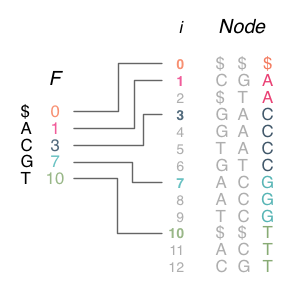
\includegraphics[width=0.5\textwidth]{f-array}}\medskip

In total we have a bitvector $L$, an array of flagged edge labels $W$, and a position array $F$ of size $\sigma$ (the alphabet size). Respectively, these take $m$ bits, $m\log{2\*\sigma}=3m$ bits (for DNA), and $\sigma \log{m} = o(m)$ bits\footnote{This is “little o” notation, which may be unfamiliar to some people. Intuitively it means “grows much slower than”, and is stricter than big O. A formal definition can be found on Wikipedia, \url{https://en.wikipedia.org/wiki/Big_O_notation\#Little-o_notation}}, given $m$ edges -- a bit over 4 bits per edge. Using appropriate structures (not detailed) we can compress this further, to around 3 bits per edge.

\subsection{Rank and Select}\label{bl-sec:ras}

Rank and select are the bread and butter of succinct data structures, because so many operations can be implemented using them alone. $\rank_c(i)$ returns the number of occurences of symbol $c$ on the closed range $[0,i]$, whereas $\select_c(
i)$  returns the position of the $i^{th}$ occurence of symbol $c$.

\medskip\centerline{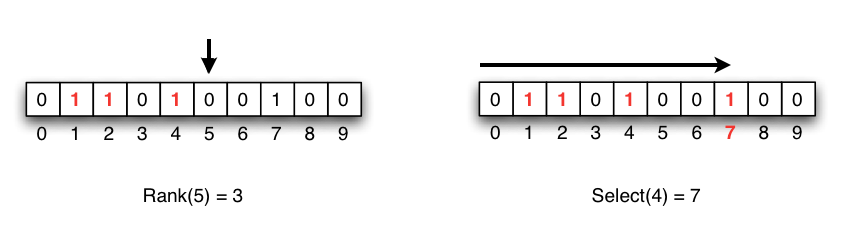
\includegraphics[width=0.9\textwidth]{ranksel}}\medskip

They are \emph{kind of} like inverse functions, although $\rank()$ is not \emph{injective}\footnote{\url{http://en.wikipedia.org/wiki/Injective_function}}, so cannot have a true inverse. For this reason, if you want to find the \emph{position} of the left-nearest $c$, you would have to use $\select()$ in orchestra with $\rank()$ (a common pattern).

Speaking of patterns of use, it may also help to keep this in mind: rank is for counting, and select is for searching, or can be thought of as an indirect addressing technique (such as addressing a node using the $L$ array). Two rank queries can count over a range, whereas two select queries can find a range. A rank and a select query can find a range where either a start point or end point are fixed.

Rank, select and standard array access can all be done in $\mathcal{O}(1)$ time when $\sigma=\textit{polylog}(N)$,\footnote{\url{http://stackoverflow.com/questions/1801135/what-is-the-meaning-of-o-polylogn-in-particular-how-is-polylogn-defined}} if represent a bitvector using the structure described by Raman, Raman and Rao in 2007~\cite{RRR07} (which I explained in an earlier blog post\footnote{\url{https://alexbowe.com/rrr}}), and for larger alphabets use the index described by Ferragina, Manzini, Makinen, and Navarro in 2006~\cite{FerManMakNav06}. In our implementation, we use modified versions to get it down to 3 bits per edge.

\subsection{Interface Overview}\label{bl-sec:int}

While it might not be obvious, these three arrays provides support for a full suite of navigation operations. An overview is given in these tables, which link to the implementation details that follow.

First, to navigate each of the edges, we define two internal functions (using rank and select calls, see Section~\ref{bl-sec:ras}):

\begin{center}
\small
\begin{tabularx}{\textwidth}{@{}lXl@{}}
\toprule  
{\bf Operation} & {\bf Description} & {\bf Complexity}\\
\midrule  
$\textit{forward}(i)$ & Return index of the \emph{last edge} of the \emph{node pointed to} by edge $i$ & $\mathcal{O}(1)$\\
$\textit{backward}(i)$ & Return index of the \emph{first edge} that \emph{points to the node} that the edge at $i$ \emph{exits}. & $\mathcal{O}(1)$\\
\bottomrule
\end{tabularx}
\end{center}

Using these two functions, we can implement the less confusing public interface below, which operate on node indexes:

\begin{center}
\small
\begin{tabularx}{\textwidth}{@{}lXl@{}}
\toprule  
{\bf Operation} & {\bf Description} & {\bf Complexity}\\
\midrule  
$\textit{outdegree}(v)$ & Return number of outgoing edges from node $v$ & $\mathcal{O}(1)$\\
$\textit{outgoing}(v,c)$ & From node $v$, follow the edge labeled by symbol $c$. & $\mathcal{O}(1)$\\	
$\textit{label}(v)$ & Return (string) label of node $v$. & $\mathcal{O}(k)$\\
$\textit{indegree}(v)$ & Return number of incoming edges to node $v$. & $\mathcal{O}(1)$\\
$\textit{incoming}(v,c)$ & Return predecessor node starting with symbol $c$, that has an edge to node $v$. & $\mathcal{O}(k\log\sigma)$\\
\bottomrule
\end{tabularx}
\end{center}

The details of the above functions are given in the following sections.

\subsection{Forward}\label{bl-sec:fwd}

In order to support the public interface, we create for ourselves a simpler way to work with edges: the complementing forward and backward functions.

Recall that all node labels are defined by predecessor edges, then we have represented each edge in two different places: the $F$ array (which is equivalent to the last column of the ``\Node'' array), and the edge array $W$. It follows that, since it is sorted, the node labels maintain the same \emph{relative order} as the edge labels. This can be seen in the following figure:

\medskip\centerline{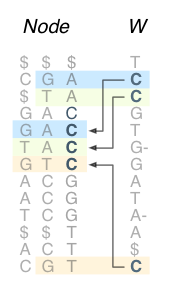
\includegraphics[width=0.3\textwidth]{fwdsetup}}\medskip

Note that the number of Cs in the last column of \Node\ is different from the number of Cs in $W$, because the first C in $W$ points to two edges. For this reason, we ignore the first edge from node GAC (although it doesn't affect the relative order). In fact, we ignore any edge that doesnt have $L[i] == 1$.

Then, following an edge is simply finding the corresponding relatively positioned node! All it takes is some creative counting, using rank and select (Section~\ref{bl-sec:ras}), as pictured below:

\medskip\centerline{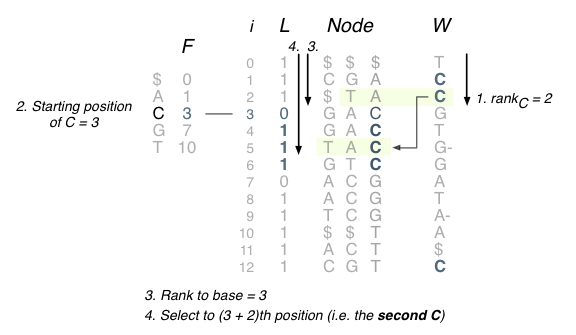
\includegraphics[width=0.8\textwidth]{fwd}}\medskip

First we access $W[i]$ to find the edge label, then calculate $\rank_C$ up to row to gives us the relative ordering of our \emph{edges} with this label. Let's call this relative index $r$. In our example we are following the 2nd C-labeled edge.

To find the 2nd occurence of C in $F$, first we need to know where the first occurence is. We can use $F$ to find that. Then we can select to the 2nd one, using the last array. Because the last array is binary only, this requires us to count how many 1s there are before the run of Cs (using rank), then adding 2 to land us at the 2nd C.

The $W$ access, rank over $W$, rank and select over $L$, accessing $F$, and the addition are all done in $\mathcal{O}(1)$ time, so forward also takes $\mathcal{O}(1)$ time.

\subsection{Backward}\label{bl-sec:bwd}

Backward is very similar to forward, but calculated in a different order: we find the relative index of the node label first, and use that to find the corresponding edge (which may not be the only edge to point to this node, but we define it to point to the first one, that is one that isn't flagged with a minus).

We can find our relative index of the node label by issuing two rank queries instead, and using select on $W$ to find the first incoming edge.

\medskip\centerline{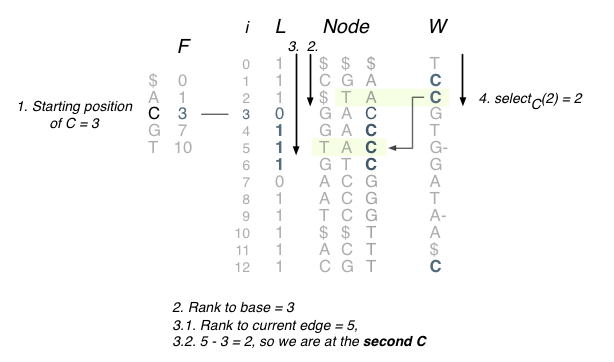
\includegraphics[width=0.8\textwidth]{bwd}}\medskip

For similar reasons to Forward this is $\mathcal{O}(1)$.

\subsection{Outdegree}\label{bl-sec:out}

This is an easy one. This function accepts a {\bf node} (not edge!) index $v$, and returns the number of outgoing edges from that node. Why did I say this was easy? Well, remember that all our outgoing edges from the same node are contiguous in our data structure. See the diagrams below, paying attention to the node ACG.

\medskip\centerline{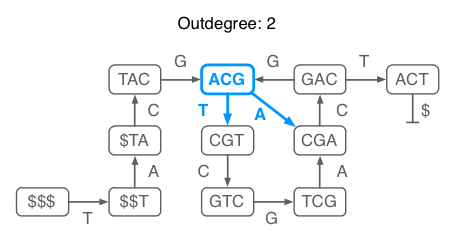
\includegraphics[width=0.6\textwidth]{outdegree-graph}\hfill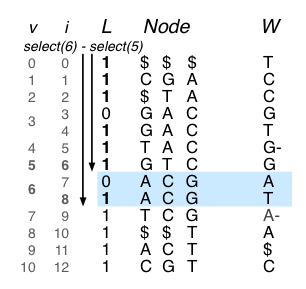
\includegraphics[width=0.4\textwidth]{outdegree-arrays}}\medskip
 
By definition (since nodes are unique and sorted), this will always be the case. We also defined our so-called ``last'' vector $L$ to have a 0 for every edge from a given node, \emph{except the last} edge. All we need to do is count how many 0s there are, then add 1. Put another way, we need to measure the distance between 1s (since the previous 1 will belong to the previous node). Since we know the node index, we can use select for that!

In the above example, we are querying the outdegree of node 6 (the 7th node due to zero-basing). First we select to find the position of the 7th 1, which gives us the last edge of that node. Then we simply subtract the position of the previous node (node 5, the 6th node): 
$\select(7)-\select(6)=8-6=2$. Boom.

Select queries can be answered in $\mathcal{O}(1)$ time, so outdegree is also $\mathcal{O}(1)$.

\subsection{Outgoing}\label{bl-sec:outg}

$\textit{Outgoing}(v,c)$ returns the target node after traversing edge $c$ from node $v$, which might not exist. The hard part is finding the correct edge index to follow; after that we can conveniently use the $\textit{forward}()$ function we defined earlier.

To ease the explanation, consider a simple bit vector 00110100. To count how many 1s there are up to and including the 7th position, we would use rank. The answer is 3, but at this stage we still don't know the position of the 3rd 1 (we can't see the bitvector). In general, it may or may not be in the 7th position. We could scan backwards, or we could just use $\select(3)$ to find the position (since this returns the first position $i$ that has $\rank(i) = 3$).

So essentially we can count how many of those edges there are before the node we are interested in, then use select to find the position. If the position is inside this nodes range (of contiguous edges), then we follow it.

\medskip\centerline{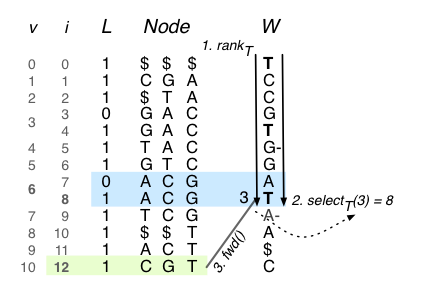
\includegraphics[width=0.6\textwidth]{outgoing}}\medskip

We complicated things a bit by separating our edges into flagged and non-flagged, so we may have to issue two of these queries (for the minus flags). The flagging is useful later in Indegree (Section~\ref{bl-sec:ind}).

In the next example, our nonflagged edge doesn't fall in our nodes range, so we make a second query. It is possible that this one will return a positive result, but in the example it doesn't. By that stage though, we can respond with by returning $-1$ to signal that the edge doesn't exist.

\medskip\centerline{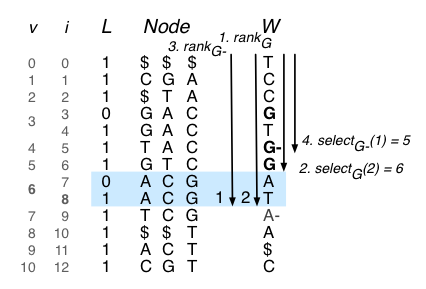
\includegraphics[width=0.6\textwidth]{outgoing-neg}}\medskip

$\textit{forward}()$ is defined to move us to the last edge of the resulting node, so the value in last will be 1. Hence, we can use rank to convert our edge index into a node index before returning it.

This is a constant number of calls to $\mathcal{O}(1)$ functions, so outgoing is also $\mathcal{O}(1)$.

\subsection{Label}\label{bl-sec:lab}

At some point (e.g.\ during traversal) we are probably going to want to print the node labels out. Let's work out how to do that.

Remember, we aren't storing the node labels explicitly. The $F$ array will come in handy: We can use the position of our node (found using select) as a reverse lookup into $F$. This can be done in constant time with a sparse bit vector, or in logarithmic time using binary search, or we can use a linear scan if our alphabet is small. In any case, lets assume it is $\mathcal{O}(1)$ time, although a linear scan might be faster in practice (fewer function calls may yield a lower constant coefficient).

\medskip\centerline{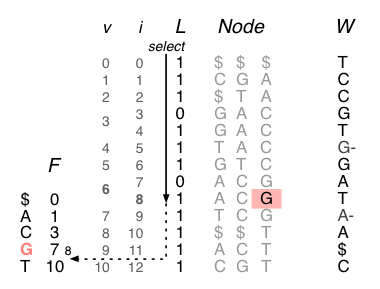
\includegraphics[width=0.5\textwidth]{last-symbol}}\medskip

In the above example, we select to node 6 (the 7th 1 in last), which gives us the last edge index (any edge will do, but the last one is the easiest to find). This happens to be row 8, so from $F$ we know that all the last symbols between on the open range $[7,10)$ are G.

Then we just use $\bwd()$ on the current edge to find an edge that pointed to this node, then rinse and repeat $k$ times.

\medskip\centerline{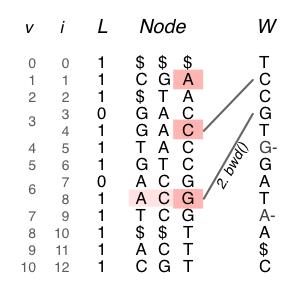
\includegraphics[width=0.4\textwidth]{label}}\medskip

\subsection{Indegree}\label{bl-sec:ind}

In a similar manner to $\textit{outdegree}$ (Section~\ref{bl-sec:out}), all we need to do is count the edges that point to the current node label. Take for example the graph:

\medskip\centerline{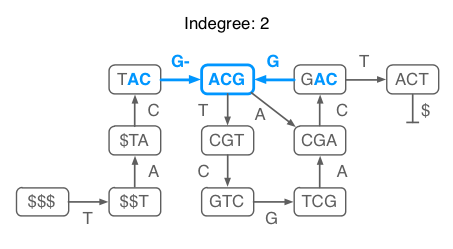
\includegraphics[width=0.7\textwidth]{indegree-graph}}\medskip

We can easily find the first incoming edge by using $\textit{backward}()$. To count the remaining edges our minus flags come in handy; In the $W$ array, the next G (non-flagged) belongs to a different node, because we defined $W$ to have minus flags if the source node has the same $k-1$ suffix (or, if same-labeled edges also share the same target node).

\medskip\centerline{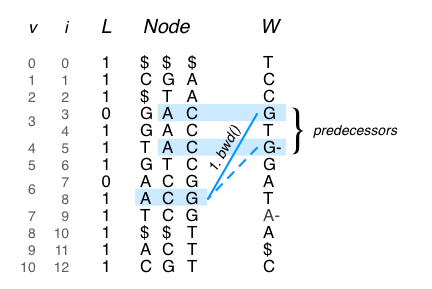
\includegraphics[width=0.55\textwidth]{indegree1}}\medskip

From here it is simple enough to do a linear scan (or even use select) until the next non-flagged edge; the maximum distance it could be is 
$\sigma^2$. For larger alphabets, a more efficient method is to use rank instead:

\medskip\centerline{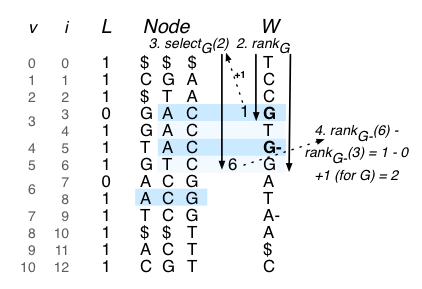
\includegraphics[width=0.55\textwidth]{indegree2}}\medskip

First we find the position of the next non-flagged G, which gives us the end point of our range (we already have the start point from the first rank). Then we use rank to calculate how many G -- there are to the end position, and subtract the initial rank value from this, giving us how many G -- occur within the range.

This is once again a constant number of $\mathcal{O}(1)$ function calls, which means $\textit{indegree}()$ is also $\mathcal{O}(1)$.

\subsection{Incoming}\label{bl-sec:inc}

Incoming, which returns the predecessor node that begins with the provided symbol, is probably the most difficult operation to implement. However, it does use approaches similar to the previous functions.

Consider this: from $\textit{indegree}()$, we already know how to count each of the predecessor nodes. We can access these nodes if we instead use select to iterate over the predecessor nodes, rather than using rank to simply count. Then, to disambiguate them by first character, we can use $\textit{label}()$.

A linear scan over the predecessors in this fashion would work, but for large alphabets we can use binary search (with a select call before each array access) to support this in $\mathcal{O}(k\log\sigma)$ time; $\log\sigma$ for the binary search, where each access is a $\mathcal{O}(1)$ select, followed by $\mathcal{O}(k)$ to compute the label.

This is demonstrated in the example below:

\medskip\centerline{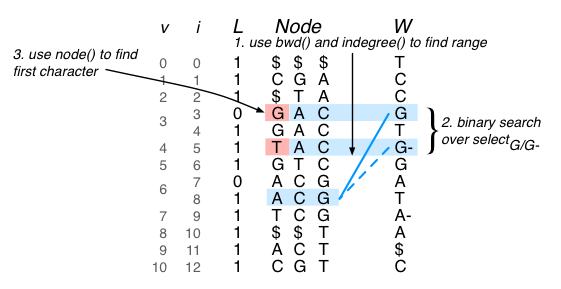
\includegraphics[width=0.7\textwidth]{incoming}}\medskip

\section{Conclusion}\label{bl-sec:conc}

In conclusion, by using memory more efficiently, hopefully the cost of genome seqeuencing can be reduced, both proliferating the technology, but also giving way to more advanced population analysis. To that end, we have described a novel approach to representing de Bruijn graphs efficiently, while supporting a full suite of navigation operations quickly. Much of the (BWT-inspired) construction can be done efficiently on disk, but we intend to improve this soon to compete with Minia.

The total space is a theoretical $m(2 + \log{\sigma} + o(1))$ bits in general, or $4m + o(m)$ bits for DNA, given $m$ edges. Using specially modified indexes we can lower this to around 3 bits per edge.

I apologize that an efficient implementation isn't available, nor have I provided experimental results. But if you found this post interesting you can get your hands dirty with the Python implementation\footnote{\url{https://github.com/alexbowe/debby/blob/0.1.1/debby.py}} I have provided. The results and efficient implementation are on their way.

%And as always, follow me on Twitter,\footnote{\url{http://www.twitter.com/alexbowe}} and feel free to send me questions, criticisms, and especially pull requests!